\section{Validation study cases}\label{validation-study-cases}

\label{sec:validation}

    The hybrid method in this paper is investigated using the well known
KVLCC2 test case. This ship was selected partly because it is a well
known test case and also because it does not have any bilge keels.
Ikeda's method contain methods to predict damping from various
components, where the bilge keels is one of them. Results from roll
decay simulations made with the hybrid method will be compared to
corresponding model test data from the SSPA Maritime Dynamics
Laboratory. From these model tests, only the total damping can be
observed. Reducing the number of components by having no bilge keels
will therefore give more insight into the remaining components.
 
            
    
    
\begin{table}[H]
\small
\center
\caption{KVLCC2 model data}
\label{tab:kvlcc2_model_data}
\begin{tabular}{lllllllll}
\toprule\addlinespace
LPP & B & ZCG & KXX & S & V & dens & ta & tf\\ 
\midrule4.706 & 0.853 & 0.274 & 0.341 & 5.981 & 0.993 & 1000.0 & 0.3059 & 0.3059\\ 

\bottomrule
\end{tabular}
\end{table}

    
 
            
    
    \begin{figure}[H]
        \begin{center}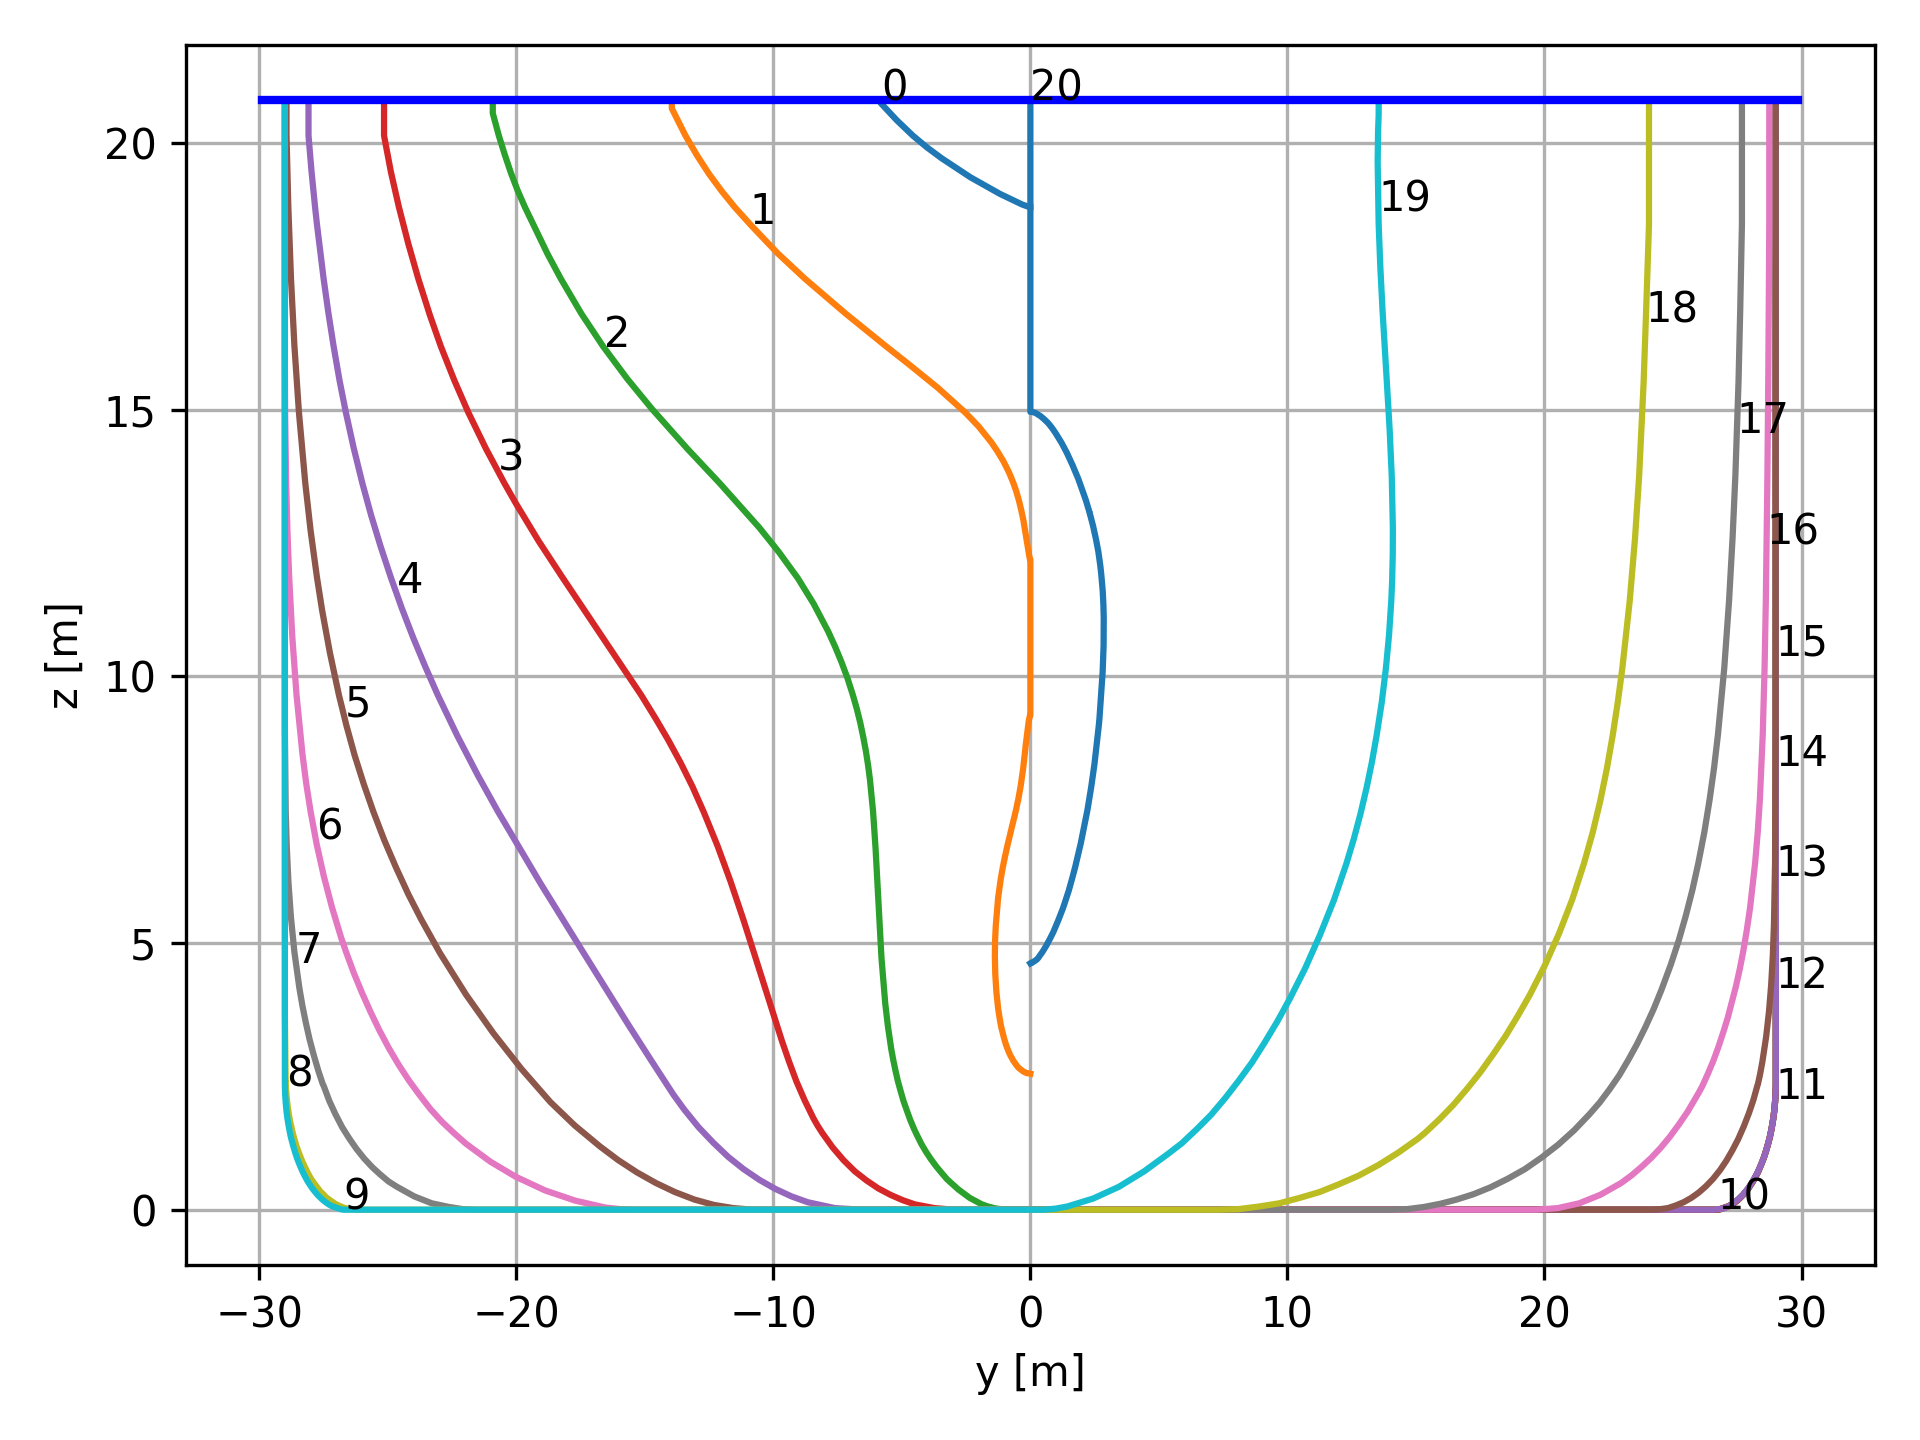
\includegraphics[width = 0.5\textwidth]{figures/body_plan.png}\end{center}
        \vspace{-1cm}
        \caption{Body plan}
        \label{fig:body_plan}
    \end{figure}
    

    